\documentclass[10pt,handout]{beamer}
\usetheme{Rochester}
\usepackage[utf8]{inputenc}
\usepackage{amsmath}
\usepackage{amsfonts}
\usepackage{amssymb}
%\setbeamertemplate{frametitle}[default][center]
\setbeamercolor{page number in head/foot}{fg=black}
\setbeamerfont{page number in head/foot}{size=\small}
\usepackage{xcolor}
\setbeamertemplate{footline}[page number]
%\beamertemplatenavigationsymbolsempty
%\setbeamertemplate{footline}[page number]
%\setbeamertemplate{footline}[frame number]
%\usepackage{siunitx}
\author{Justin Anguiano, Margaret Lazarovits}
\title{\textcolor{red}{Classifying Charged Particles} from High Energy Collisions at the \textcolor{red}{L}arge \textcolor{red}{H}adron \textcolor{red}{C}ollider }


%\setbeamercovered{transparent} 
%\setbeamertemplate{navigation symbols}{} 
%\logo{} 
\institute{University of Kansas} 
\date{\today} 
%\subject{} 
\begin{document}

\begin{frame}
\titlepage
\end{frame}



\begin{frame}{Introduction}
Overall project goal:\\
\quad \quad \\
\begin{itemize}
\item[] Classify particles better to assist with search for particle
 darkmatter
\item[] \quad
\end{itemize}
Specific focus:
 \begin{itemize}
	
	\item[] \quad
	\item[-] Discrminate low momentum true muons($\mu^\pm$) from particles imitating muons in reconstruction
\end{itemize}


\end{frame}

\begin{frame}{Motivation}
\textbf{KU CMS analysis in progress} -- \textcolor{red}{searching for particle dark matter via compressed SUSY models}\\

\begin{columns}
\begin{column}{0.5\textwidth}
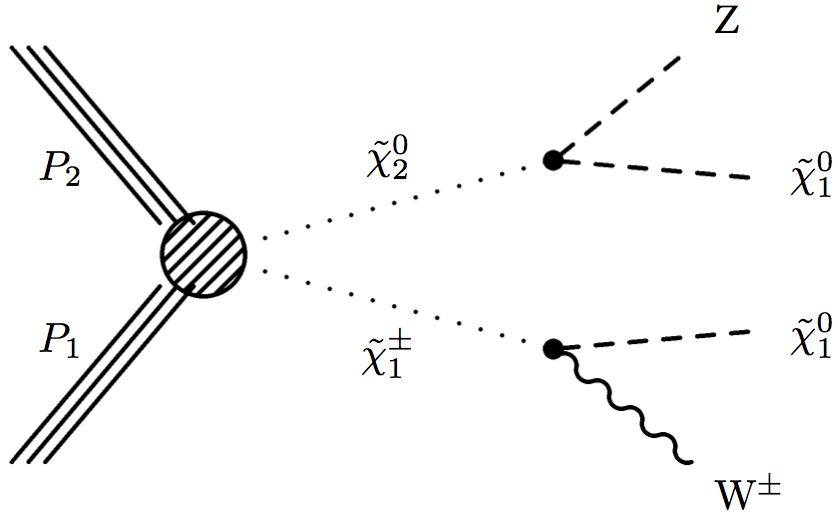
\includegraphics[scale=.75]{TChiWZ.png}
\end{column}
\begin{column}{0.5\textwidth}
\begin{itemize}
\small
\item Protons $P_1$, $P_2$ collide producing SUSY $\tilde \chi^{\pm}_1$,$\tilde \chi_2$ 
\item SUSY $\tilde \chi^{\pm}_1$,$\tilde \chi_2$ decays to D.M. $\tilde \chi^0_1$ and known particles $W^\pm$,$Z$
\item $W^\pm$,$Z$ immediately decay into charged particles($\mu^\pm$) that we see in the detector
\end{itemize}
\end{column}
\end{columns}
\small
\quad \quad \\
A compressed scenario implies $\tilde \chi^{\pm}_1$,$\tilde \chi_2$ and  $\tilde \chi^0_1$ are very close in rest mass\\
\quad \quad \\
With compression the decay products of $\tilde \chi^{\pm}_1$,$\tilde \chi_2$ are soft (low momentum), including ending charged particles\\
\quad \quad \\
The current CMS detector is less optimized for correctly identifying soft $\mu^\pm$\\
\quad \quad \\
If we can optimize soft charged particle classification, we have a better chance of discovering compressed $\tilde \chi^{\pm}_1$,$\tilde \chi_2$, and $\tilde \chi^0_1$

\end{frame}

\begin{frame}{Anatomy of an Event}
\begin{columns}
\begin{column}{0.5\textwidth}
The ``physics workflow" 
\begin{itemize}
\small
\item An event consists of \textcolor{red}{colliding protons} which \textcolor{red}{produces particles} showering outward(transverse)\\

\item We \textcolor{red}{measure the energy and momentum} of all the visible particles in the event

\item There are 100s of charged particles per event\\

\item \textcolor{red}{Reconstruct intermediate or invisible particles} through momentum and energy conservation
\end{itemize}

\end{column}
\begin{column}{0.5\textwidth}
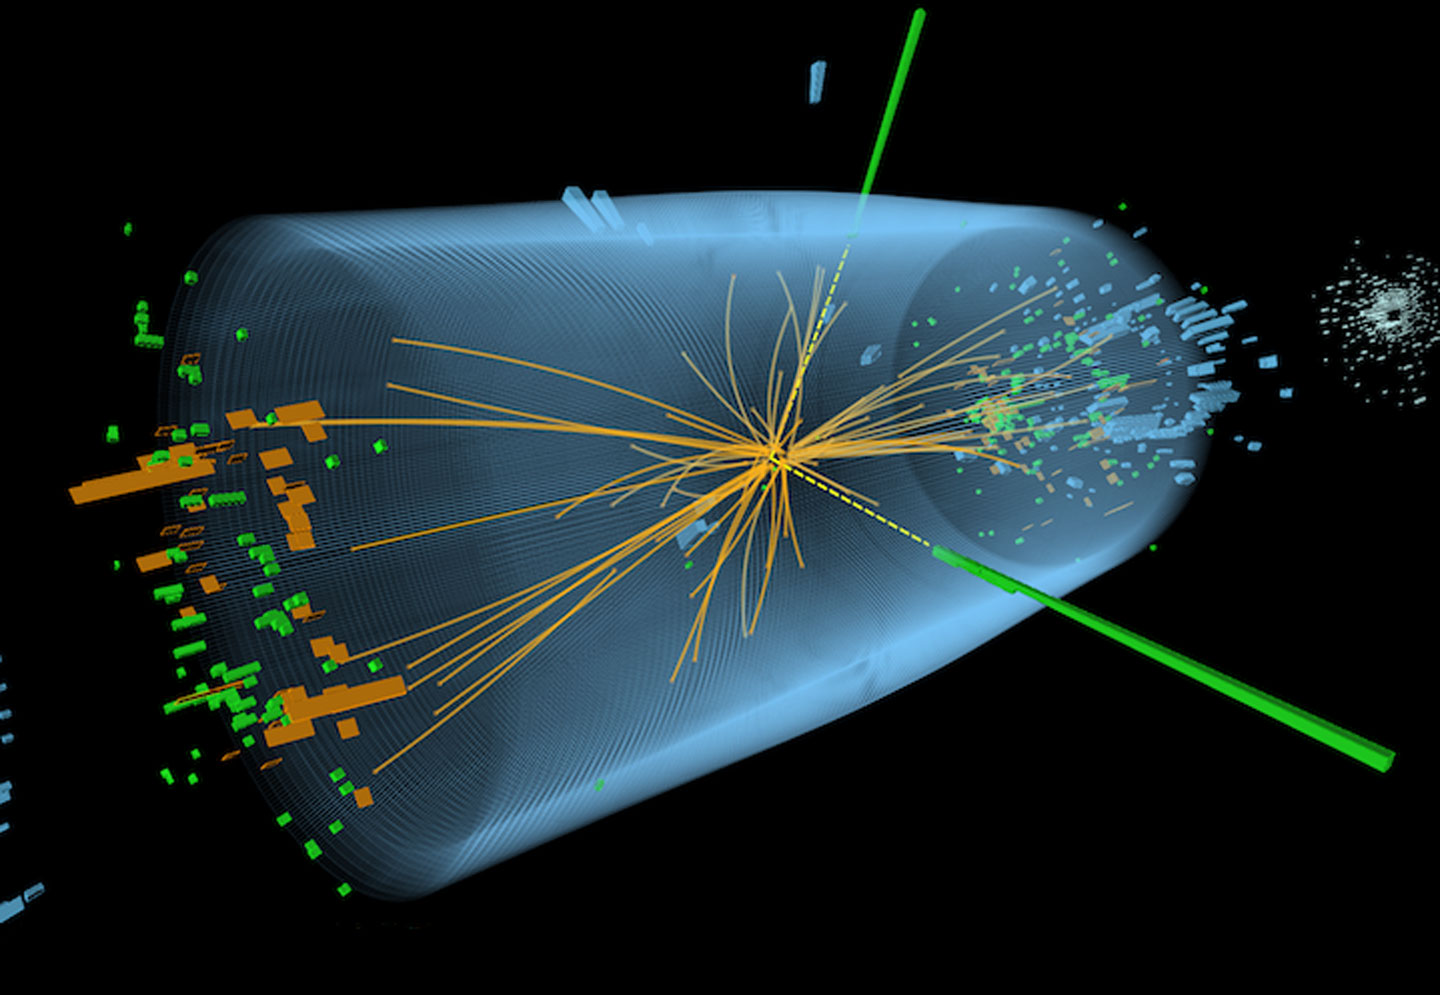
\includegraphics[scale=.12]{cms-event.jpg}\\
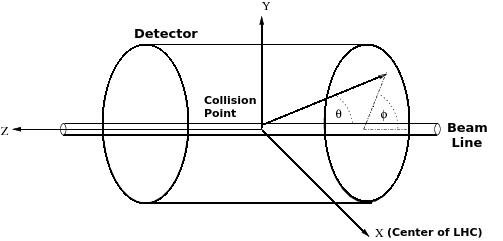
\includegraphics[scale=.2]{coords.png}
\end{column}
\end{columns}



\end{frame}

\begin{frame}{Charged Particle Reconstruction}
\begin{columns}
\begin{column}{0.5\textwidth}
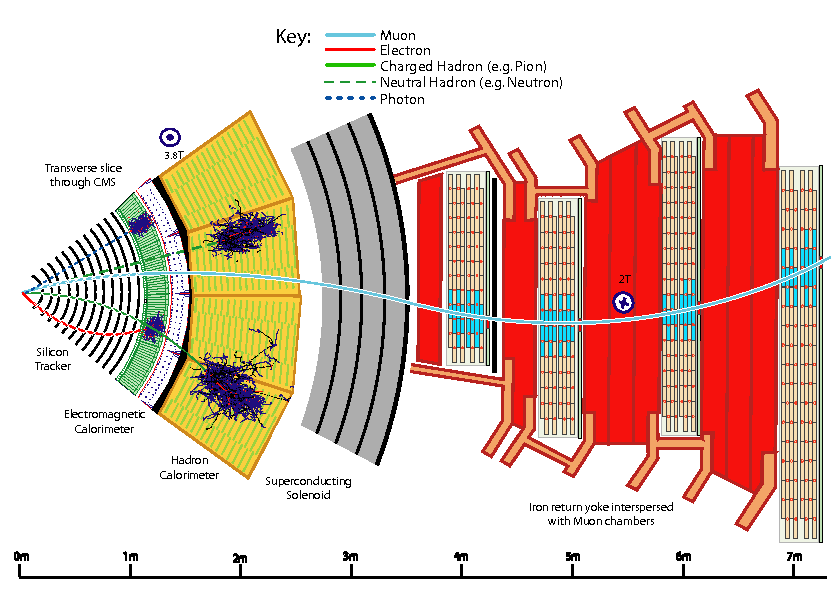
\includegraphics[scale=0.2]{particles.png}\\
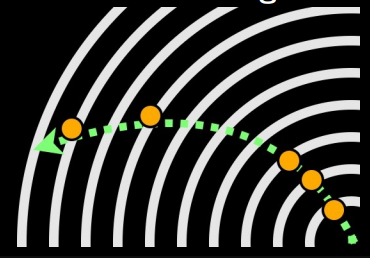
\includegraphics[scale=0.2]{trackreco.png}
\end{column}
\begin{column}{0.5\textwidth}
\small
Charged particles bend in Mag. field and create ``tracks"\\
\quad \quad \\
Tracks are connecting the dots: ``hits'' that are fit with a curve \\
\quad \quad \\
Main particle of interest is the Muon($\mu^\pm$)\\
\scriptsize
\quad	-- at high energies $\mu$ is easily correctly identified\\
\quad	-- low energies leaves room for ambiguity\\
\small
\quad \quad \\
Sometimes other particles can be reconstructed incorrectly as a muon\\
\scriptsize
\quad	-- Common fakes: Pion($\pi^\pm$), Electron($e^\pm$), Kaon($K^\pm$), Proton($p$), or non physical junk particles\\
\quad	-- created from punch through\\
\quad	-- junk particles are a result of hit combinatorics\\


\end{column}
\end{columns}



\end{frame}

\begin{frame}{ML Model Introduction}
\begin{itemize}
\item Deep Neural Network\\

\item Use fully simulated processes to get collections of reconstructed muons\\

\item Reconstructed muons contains both true(Gen.) muons and fakes.\\
\begin{itemize}
\item This generator information will be our truth, or label, for the network
\item Some particles cant be matched because they are junk -- this is unmatched label
\end{itemize}

\item Utilize two types of classification\\ 
\begin{itemize}
\item[1.] ID true muons against everything else [Unmatched,$\pi$,$K$,$p$] -- binary classification\\

\item[2.] ID every particle simultaneously -- 5 classes logistic
\end{itemize}
\item Network inputs are measured quantities and track quality metrics

\end{itemize}
\end{frame}




\begin{frame}{Data Preparation \& Network Input}
\begin{columns}
\begin{column}{0.5\textwidth}
Data Preparation
\begin{itemize}
\item Taking data from ROOT trees and converted it to pandas DataFrames
\item Evenly sampled among classes from different MC generated processes
\begin{itemize}
\item Each process produces kinematically different muons with different origins
\end{itemize}
\item One-hot encoded the classes for categorical output
\item Normalized data
\end{itemize}
\end{column}

\begin{column}{0.5\textwidth}
Network Inputs
\begin{itemize}
\item Minimal model: variables that can ID a good muon (cut-based benchmark)
\item Complex model: energy, position, track information (MVA benchmark)
\item Custom: combination of the two
\item Evaluate performance with accuracy and loss values and efficiency and ROC plots
\end{itemize}
\end{column}
\end{columns}
\end{frame}



\begin{frame}{Network Architecture \& Training Stats}
\begin{columns}
\begin{column}{0.5\textwidth}
Architecture
\begin{itemize}
\item 4 hidden layers
\item 128 neurons/layer
\item ReLU activation
\item Softmax activation on last layer
\item Adam optimizer
\item Categorical cross entropy loss
\end{itemize}
\end{column}

\begin{column}{0.5\textwidth}
Training
\begin{itemize}
\item 35/65 test/training split
\item 10/90 validation/training split
\item 100 epochs
\item 256 batch size
\end{itemize}
\end{column}
\end{columns}
\end{frame}


\begin{frame}{Results: Binary Classifier}
Network statistics \\
\quad \quad \\
\begin{columns}
\begin{column}{0.3\textwidth}
Training
\begin{itemize}
\small
\item Accuracy: 0.9593
\item Loss: 0.1060
\end{itemize}
\end{column}
\begin{column}{0.3\textwidth}
Validation
\begin{itemize}
\small
\item Accuracy: 0.9299
\item Loss: 0.2374
\end{itemize}
\end{column}
\begin{column}{0.3\textwidth}
Test
\begin{itemize}
\small
\item Accuracy: 0.9244
\item Loss: 0.2728
\end{itemize}
\end{column}
\end{columns}
\end{frame}


\begin{frame}{Results: Binary Classifier}
\centering
\quad \\ \quad \\
Muon Classification \\
\begin{itemize}
\centering
\item Efficiency: 95.274\%
\item Purity: 91.540\%
\end{itemize}
\quad \quad \\
Efficiency = $\frac{TP}{TP+FN}$ \\
\quad \\
Purity = $\frac{TP}{TP+FP}$
\end{frame}

\begin{frame}{Results: Binary Classifier}
\centering
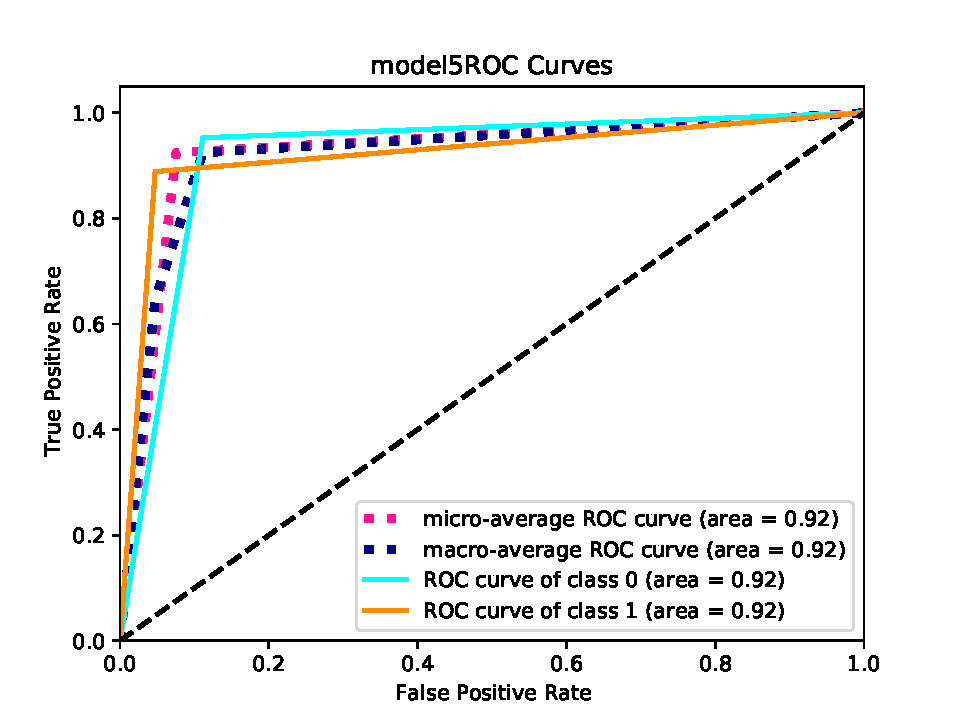
\includegraphics[scale=0.6]{model5_ROCcurves.pdf}
\end{frame}


\begin{frame}{Results: Multiclass Classifier}
Network statistics \\
\quad \quad
\begin{columns}
\begin{column}{0.3\textwidth}
Training
\begin{itemize}
\small
\item Accuracy: 0.6854
\item Loss: 0.7739
\end{itemize}
\end{column}
\begin{column}{0.3\textwidth}
Validation
\begin{itemize}
\small
\item Accuracy: 0.5323
\item Loss: 1.2388
\end{itemize}
\end{column}
\begin{column}{0.3\textwidth}
Test
\begin{itemize}
\small
\item Accuracy: 0.5330
\item Loss: 1.2864
\end{itemize}
\end{column}
\end{columns}
\end{frame}

\begin{frame}{Results: Multiclass Classifier}
\begin{columns}
\begin{column}{0.5\textwidth}
Muon Classification
\begin{itemize}
\item Efficiency: 84.032\%
\item Purity: 87.322\%
\end{itemize}
Pion Classification
\begin{itemize}
\item Efficiency: 17.401\%
\item Purity: 41.398\%
\end{itemize}
\end{column}
\begin{column}{0.5\textwidth}
Kaon Classification
\begin{itemize}
\item Efficiency: 21.601\%
\item Purity: 33.932\%
\end{itemize}
Proton Classification
\begin{itemize}
\item Efficiency: 11.496\%
\item Purity: 4.088\%
\end{itemize}
\end{column}
\end{columns}
\centering
\quad  \\
\quad  \\
\quad \quad \\
Efficiency = $\frac{TP}{TP+FN}$ \\
\quad \\
Purity = $\frac{TP}{TP+FP}$
\end{frame}




\begin{frame}{Results: Multiclass Classifier}
\centering
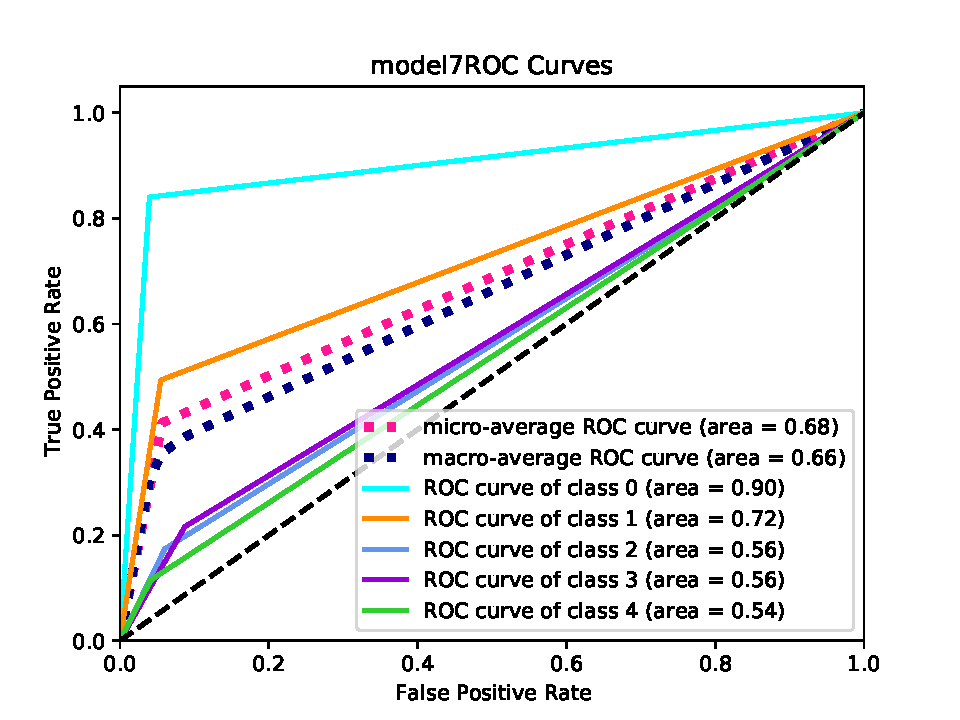
\includegraphics[scale=0.6]{model7_ROCcurves.pdf}
\end{frame}


\begin{frame}{Results: Efficiencies}
\centering
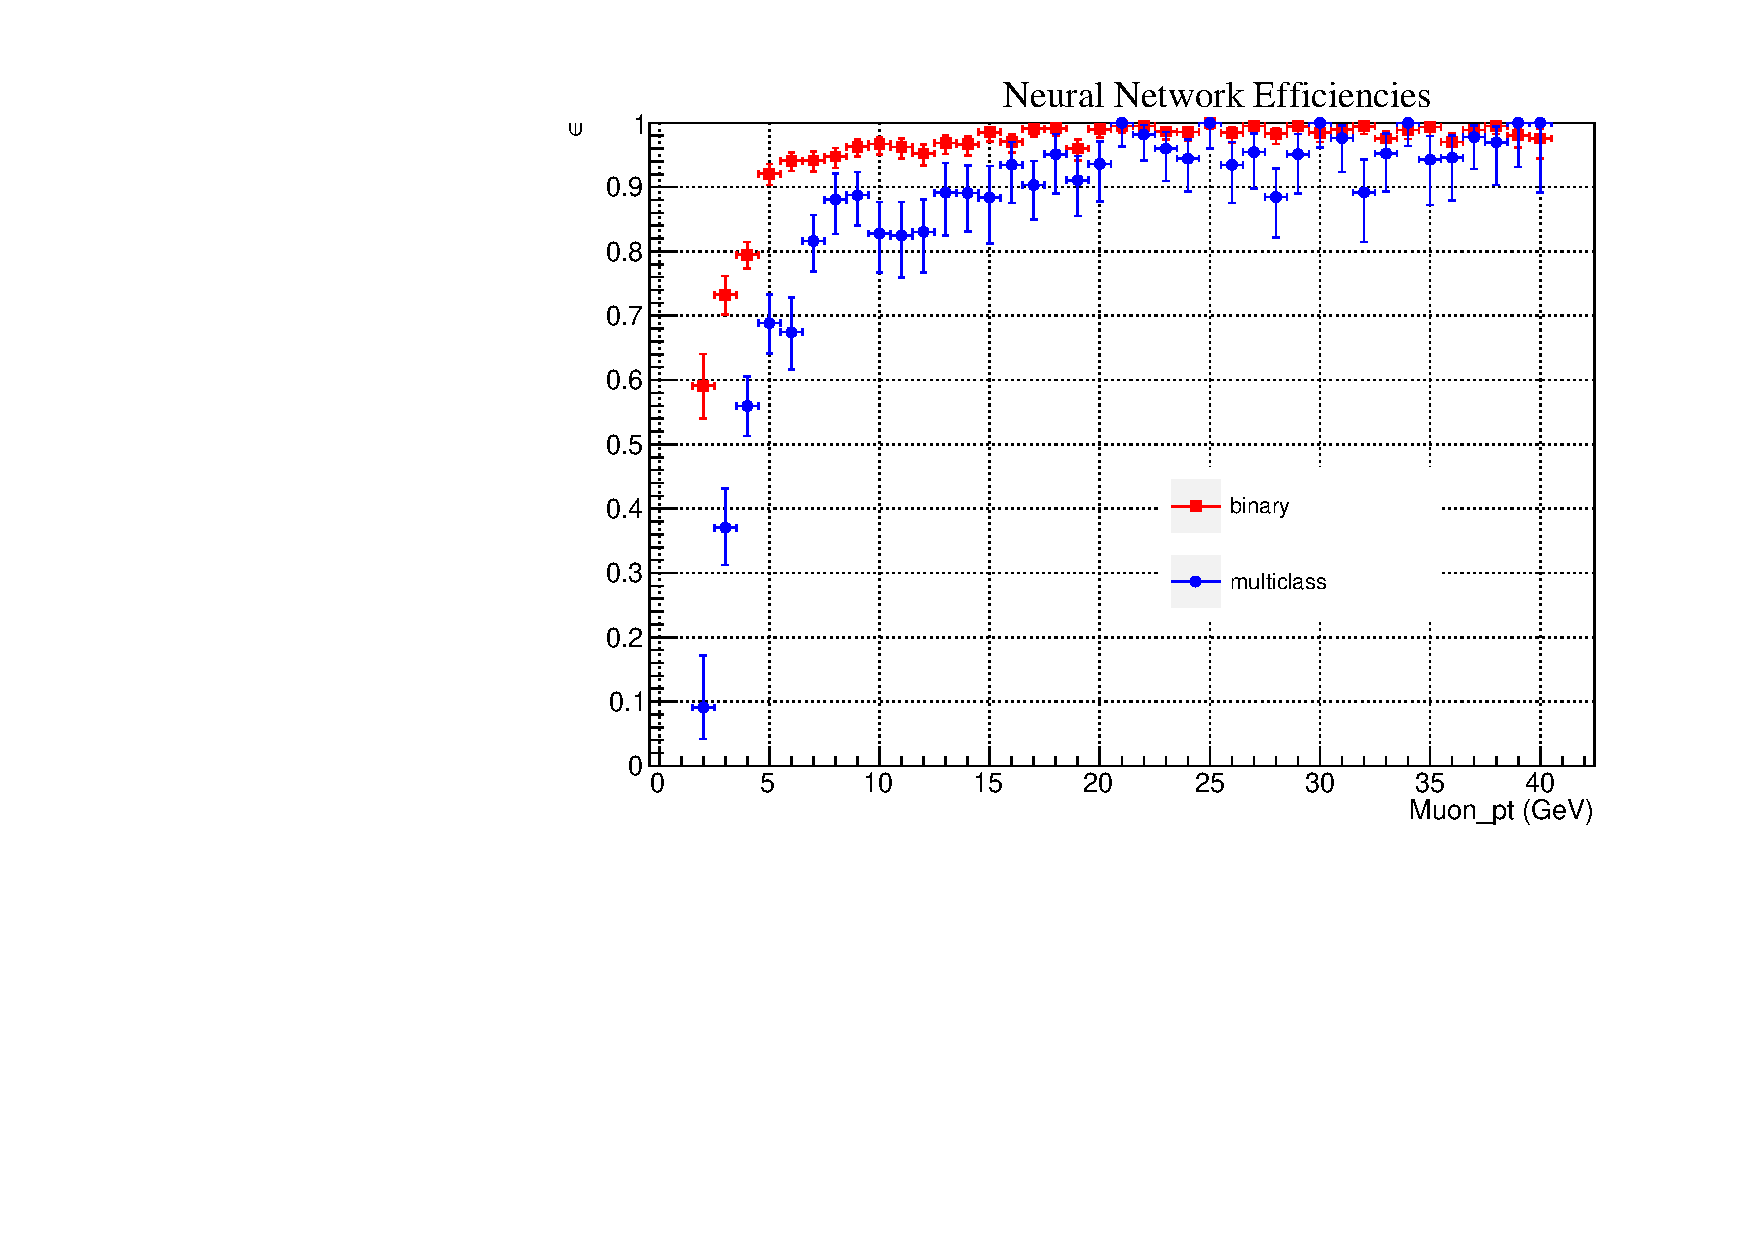
\includegraphics[scale=0.5]{NN_efficiencies.pdf}

$\epsilon$ = \# true muons that pass ID/\# true muons
\end{frame}

\begin{frame}{Results: Purities}
\centering
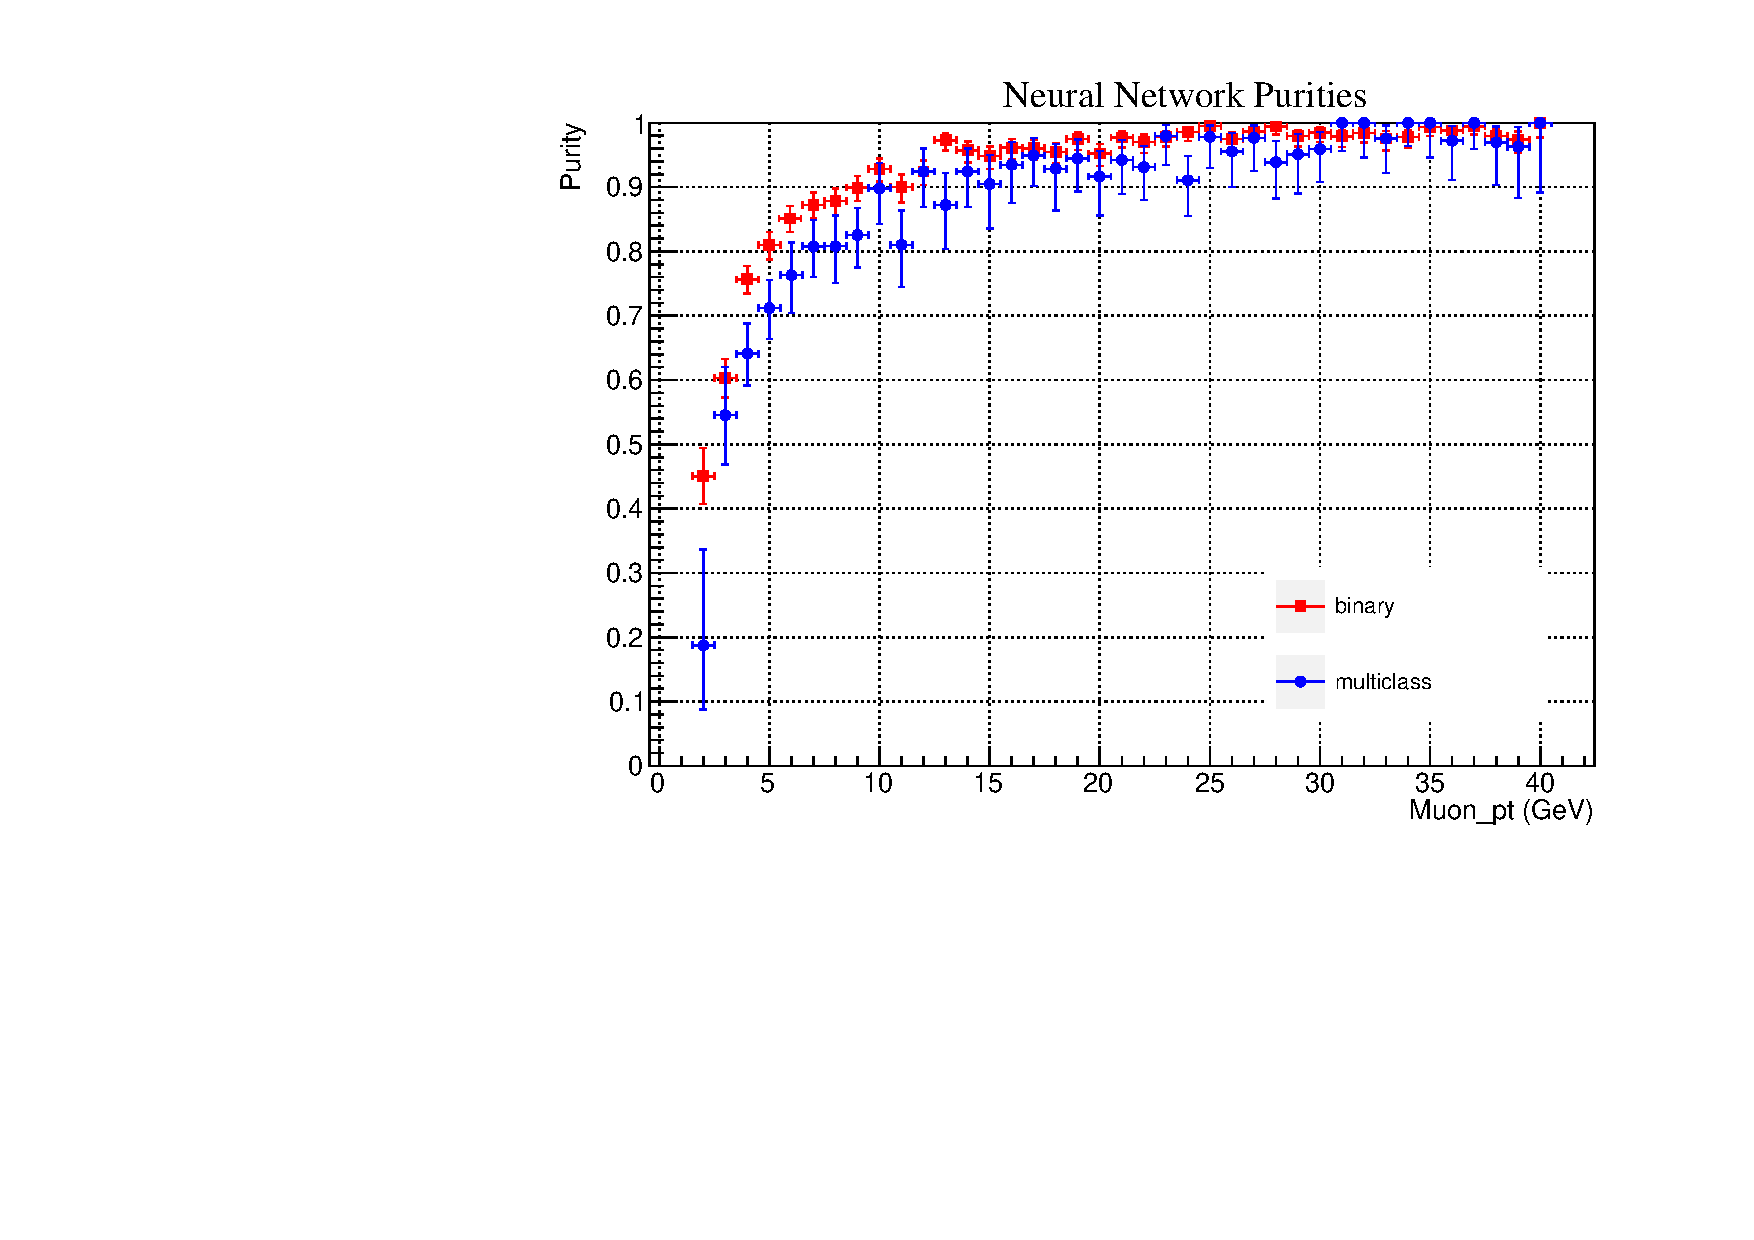
\includegraphics[scale=.5]{NN_purities.pdf}

Purity = \# true muons that pass ID/ \#reconstructed muons
\end{frame}

\begin{frame}{Benchmark Model}
Current techniques to identify low momentum muons are a cut-based ID and a multi-variate analysis (MVA) that uses a gradient boosted regression forest
\quad \\
\begin{itemize}
\item Cut-based ID - uses cuts on a few key variables
\item Soft MVA - more complex, uses energy and track information
\end{itemize}
\quad \\
\quad \\
Evaluation Statistics
\begin{itemize}
\item Efficiency $\epsilon$ = \# true muons that pass ID/\# true muons
\item Purity = \# true muons that pass ID/ \#reconstructed muons
\end{itemize}
\end{frame}




\begin{frame}{Benchmark Model: Efficiency}
\centering
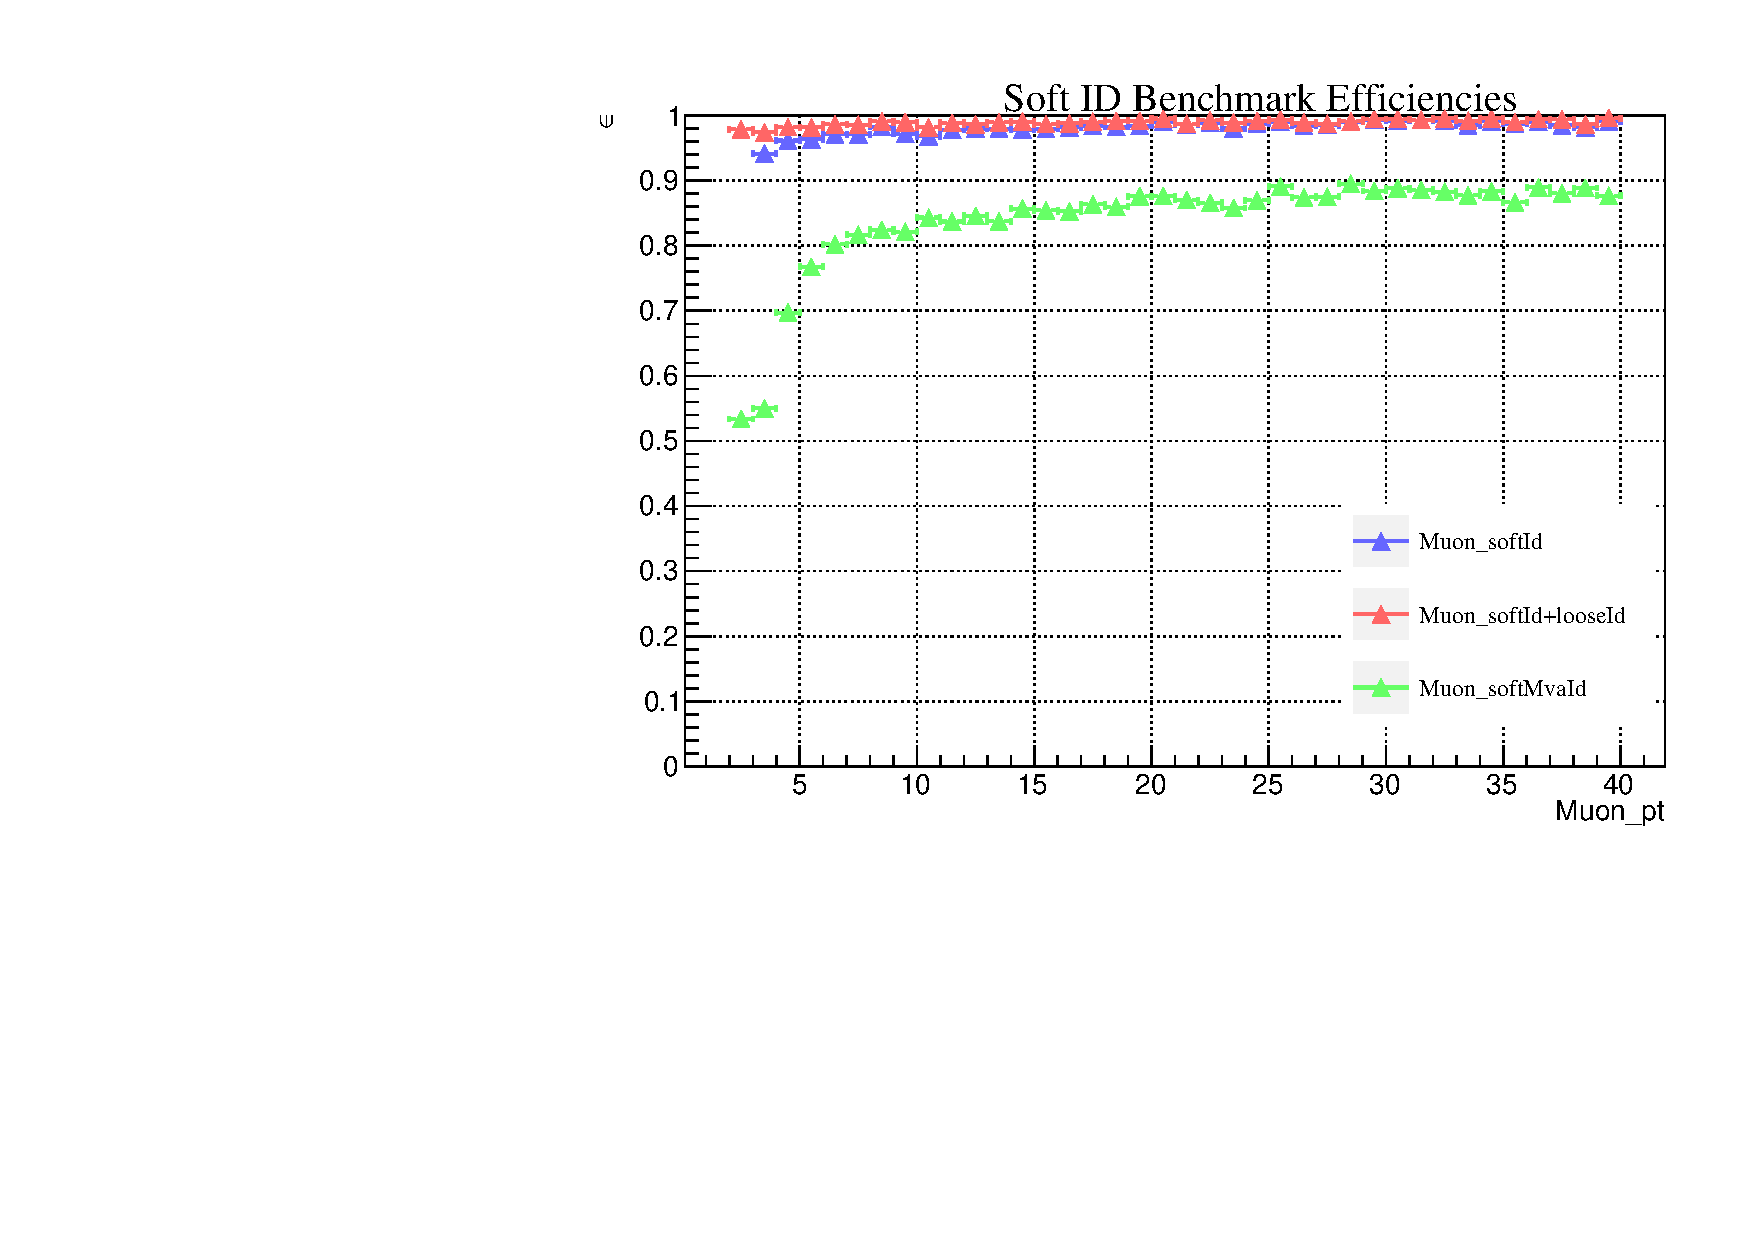
\includegraphics[scale=.5]{benchmarkEfficiency_TTjets.pdf}

$\epsilon$ = \# true muons that pass ID/\# true muons
\end{frame}


\begin{frame}{Results: Efficiencies}
\centering
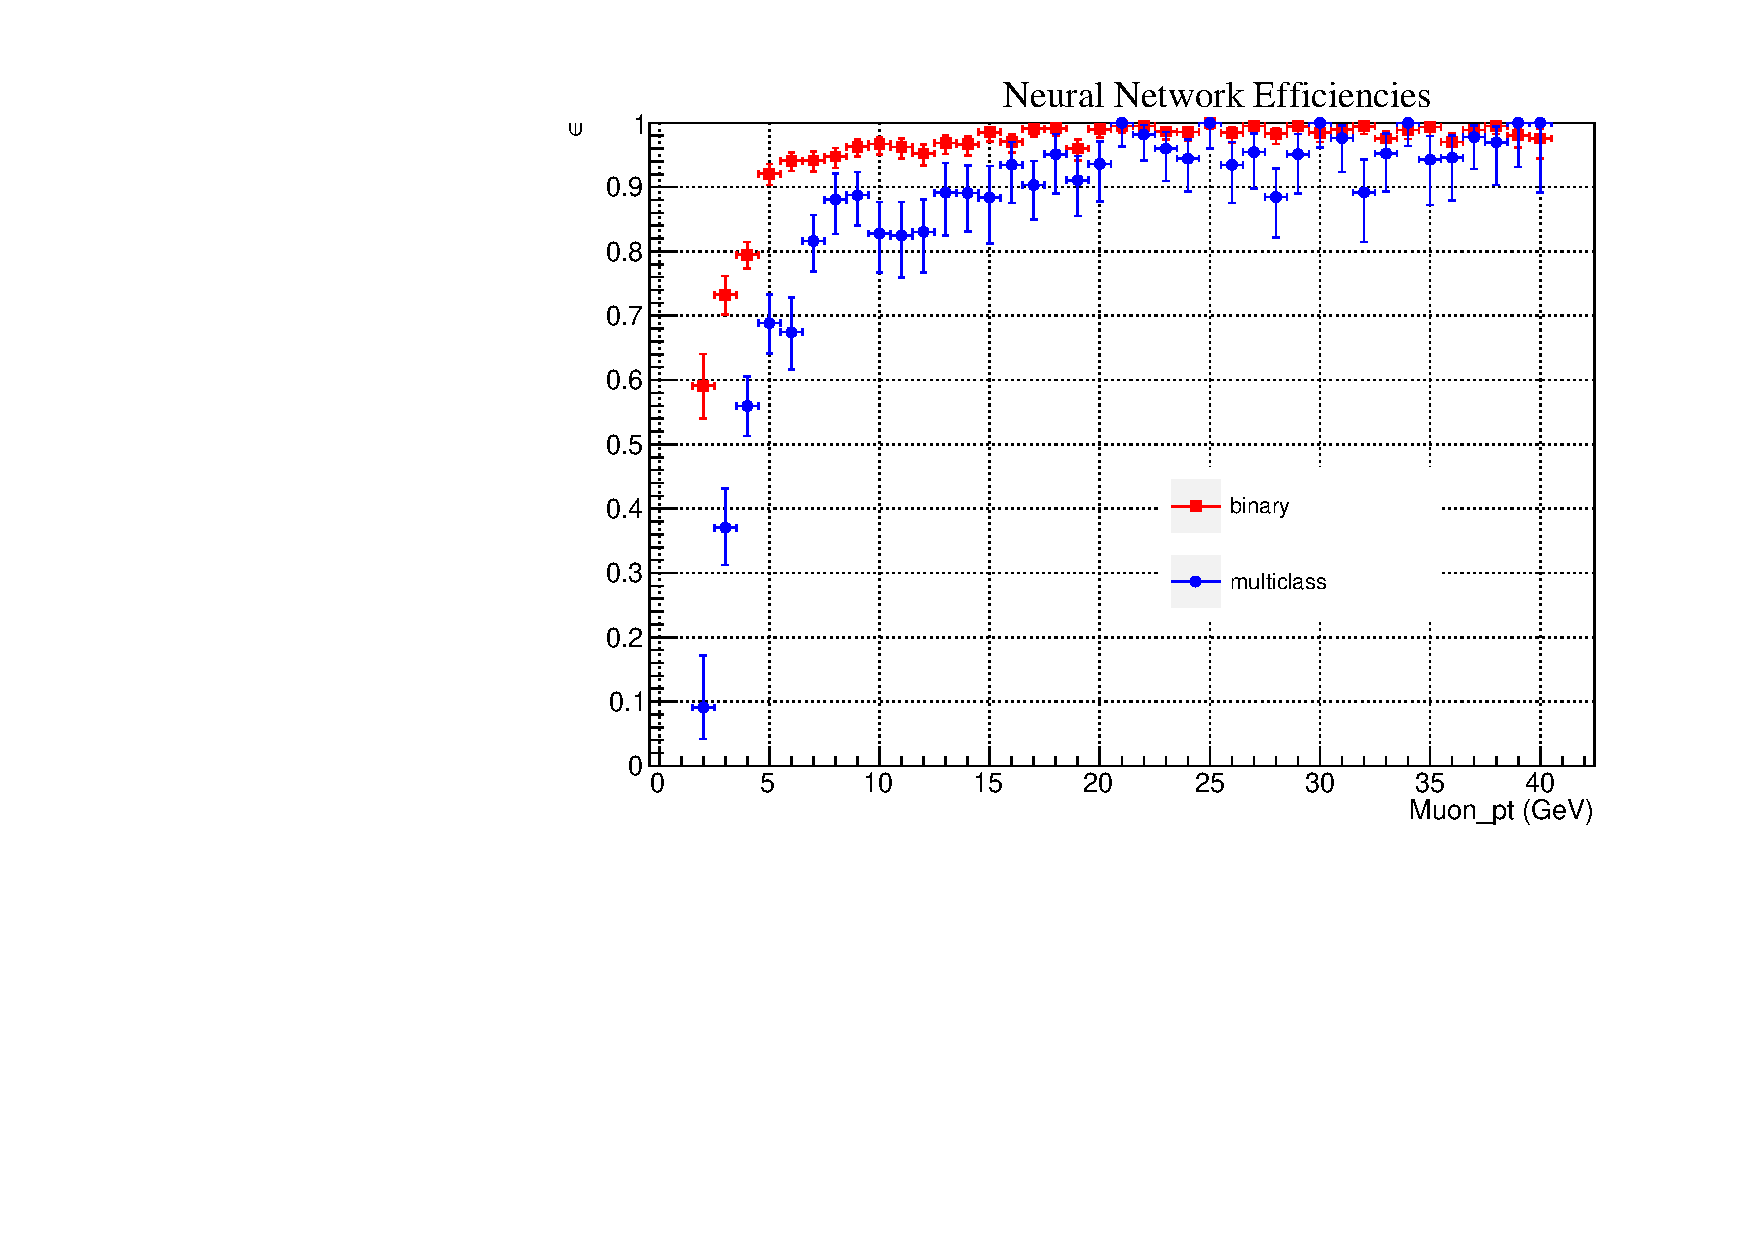
\includegraphics[scale=0.5]{NN_efficiencies.pdf}

$\epsilon$ = \# true muons that pass ID/\# true muons
\end{frame}


\begin{frame}{Benchmark Model: Purity}
\centering
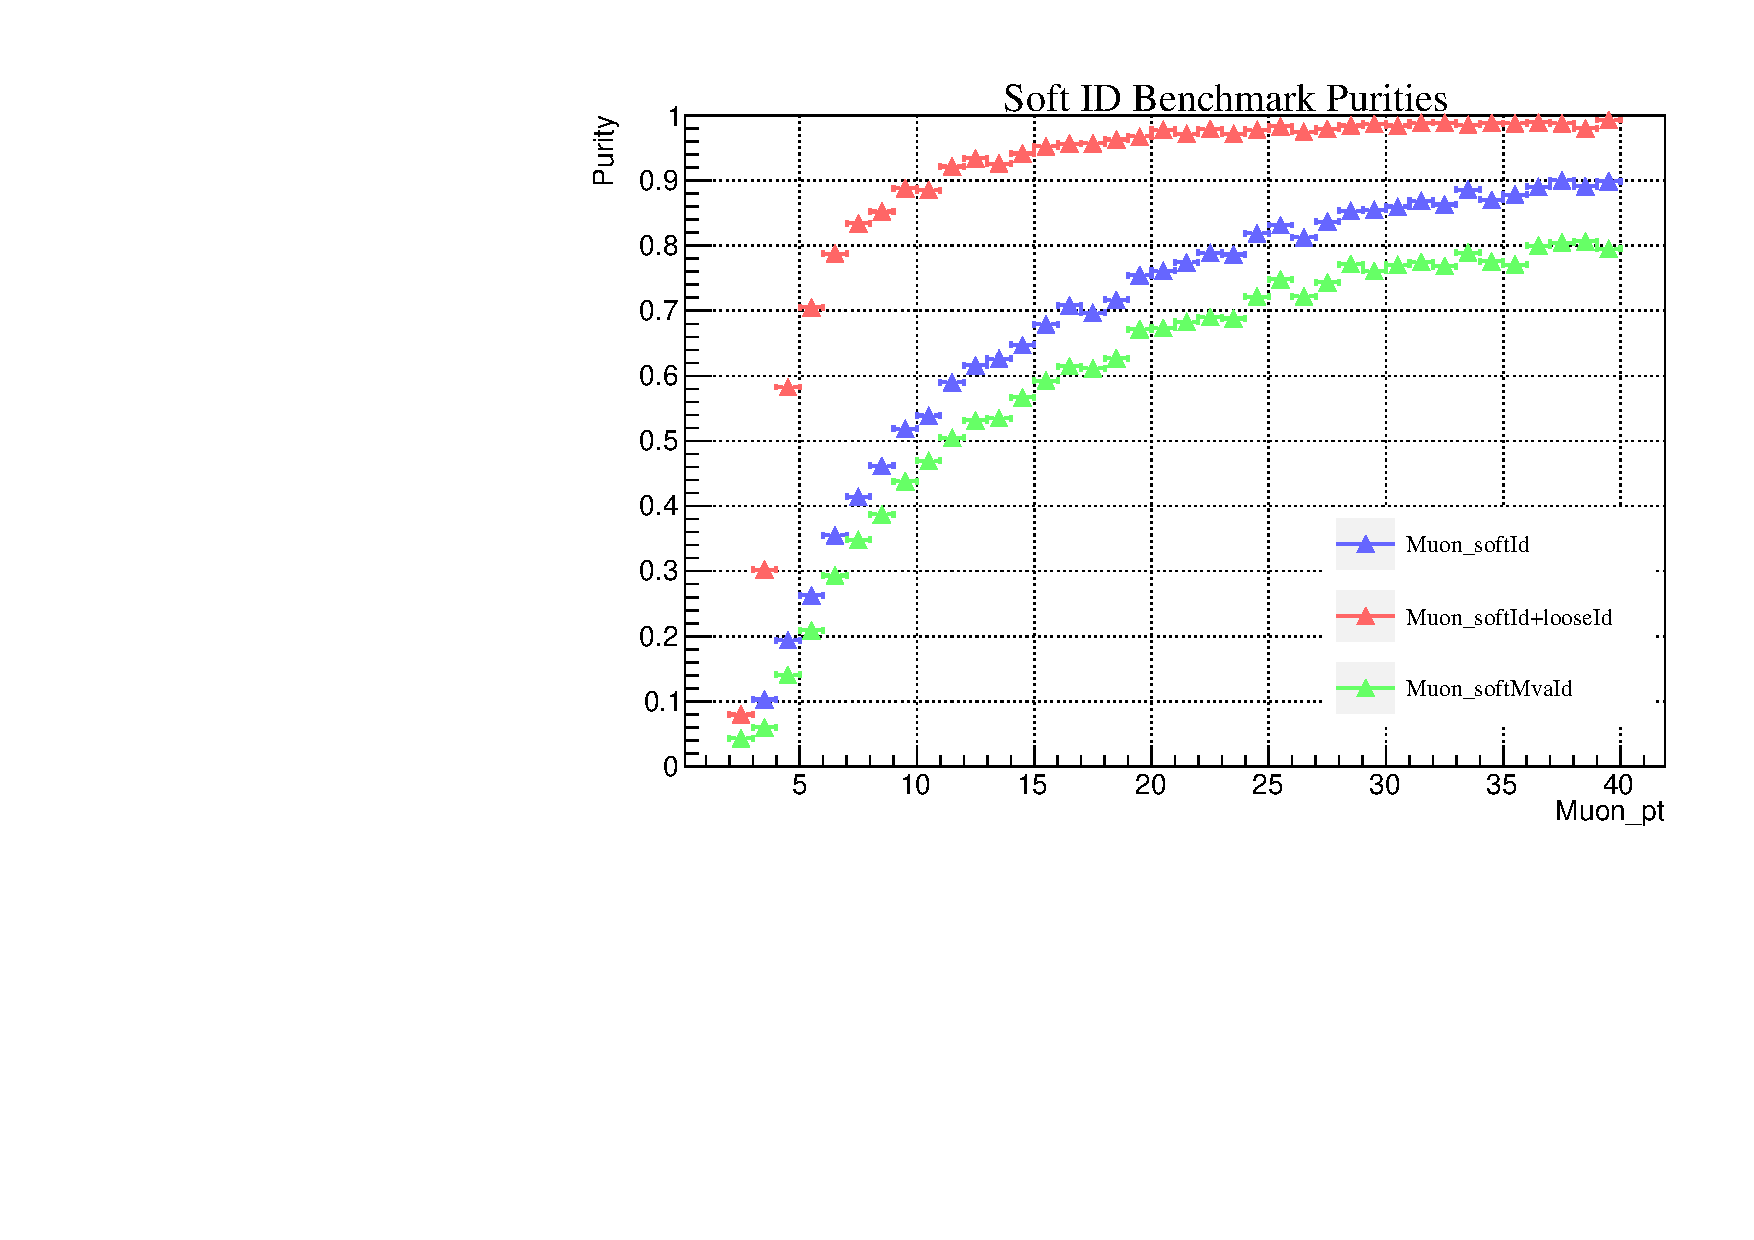
\includegraphics[scale=.5]{benchmarkPurity_TTjets.pdf}

Purity = \# true muons that pass ID/ \#reconstructed muons
\end{frame}


\begin{frame}{Results: Purities}
\centering
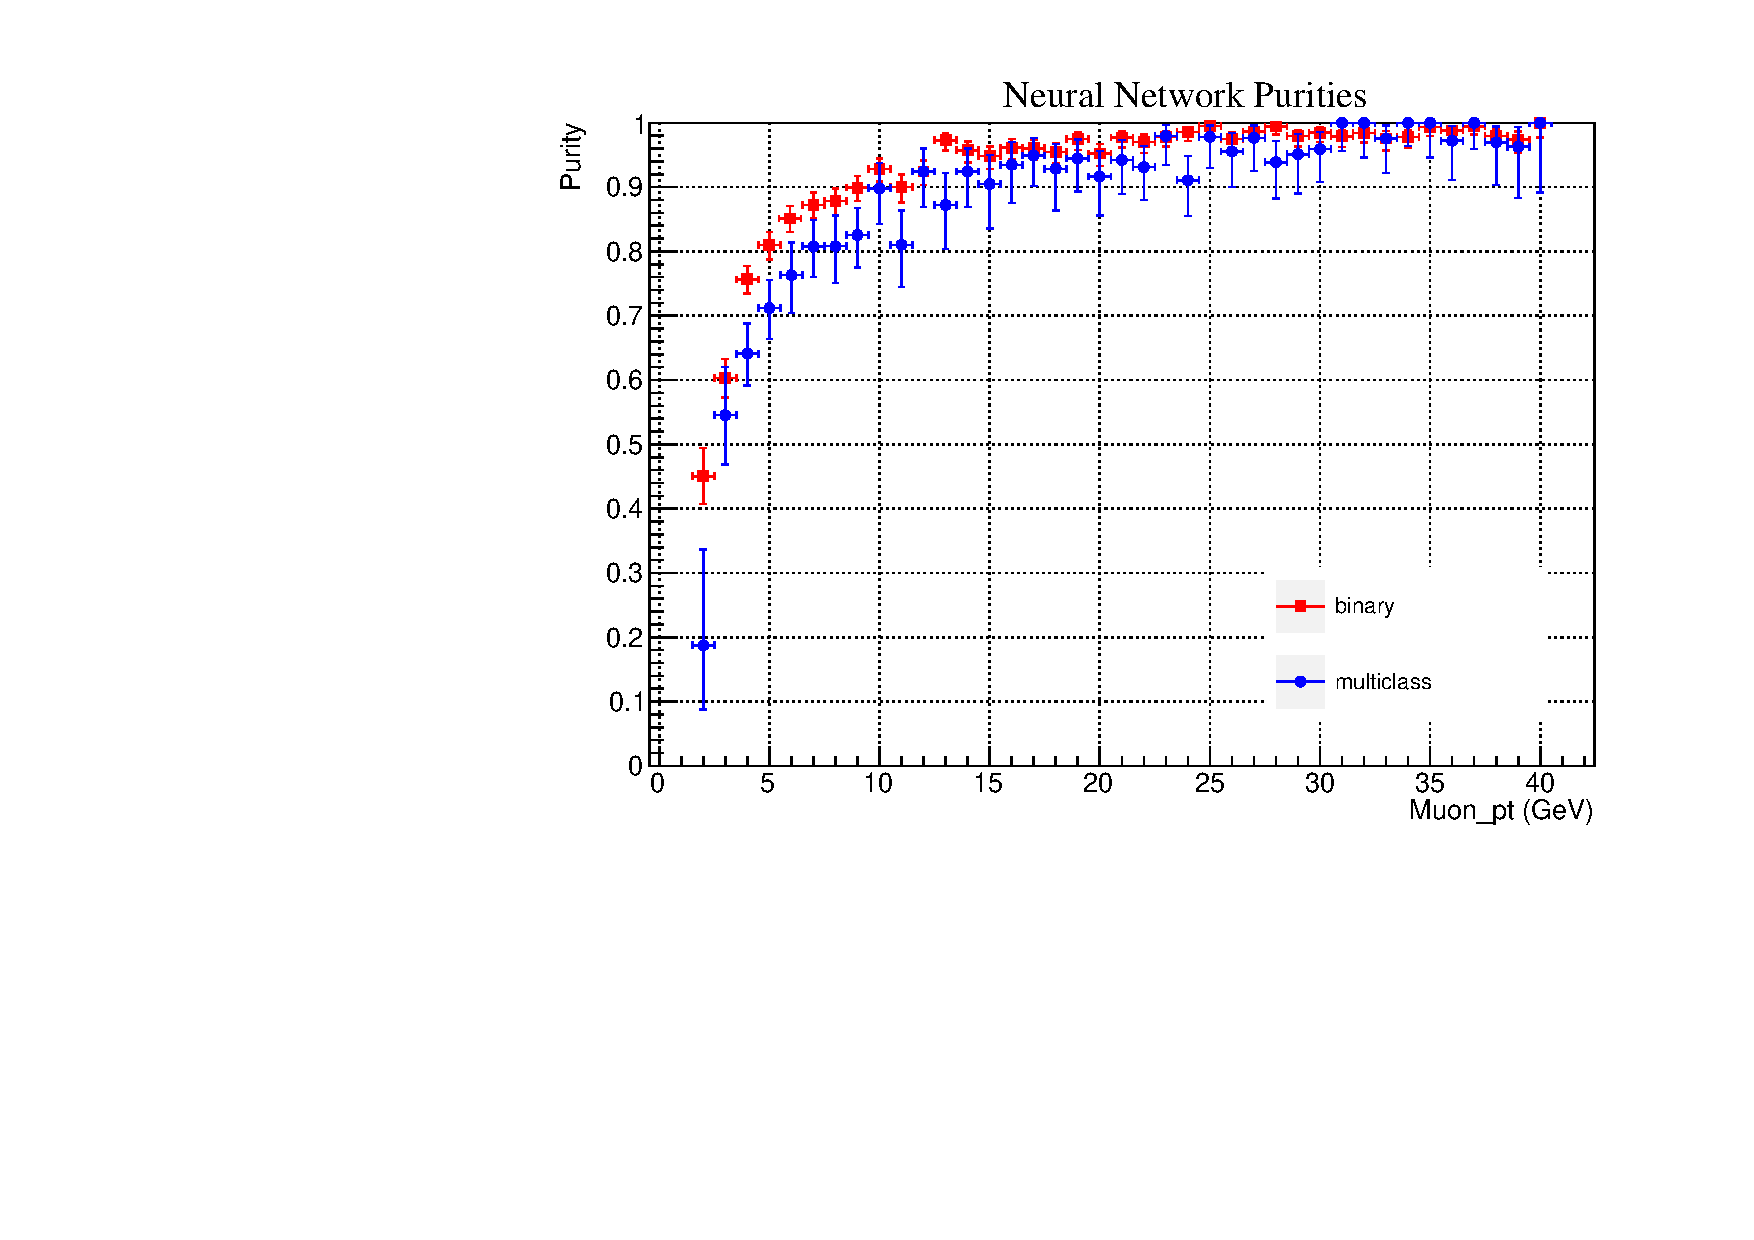
\includegraphics[scale=.5]{NN_purities.pdf}

Purity = \# true muons that pass ID/ \#reconstructed muons
\end{frame}


\begin{frame}{Summary}
Goal: correctly classify low momentum muons from proton-proton collisions at the LHC with a neural network
\quad \\
\quad \\
Results
\begin{itemize}
\item kicked ass
\item we did it lads
\item binary classifier more successful at classifying electrons than multiclass output
\begin{itemize}
\item higher efficiency and purity
\end{itemize}
\item both models competitive with current classification techniques in efficiency
\item both models have similar or higher purity than current classification techniques
\end{itemize}
\quad \\
\quad \\
Future work: integrate classifier into searches for Supersymmetry to find Dark Matter candidates
\quad \\
\quad \\
Project Repository: \url{https://github.com/Jphsx/KUSoftMVA}
\end{frame}

\begin{frame}{Thank You!}
\centering
Questions?
\end{frame}

\begin{frame}{}
\centering
Backup
\end{frame}






\begin{frame}{Benchmark Model Performances}
\centering
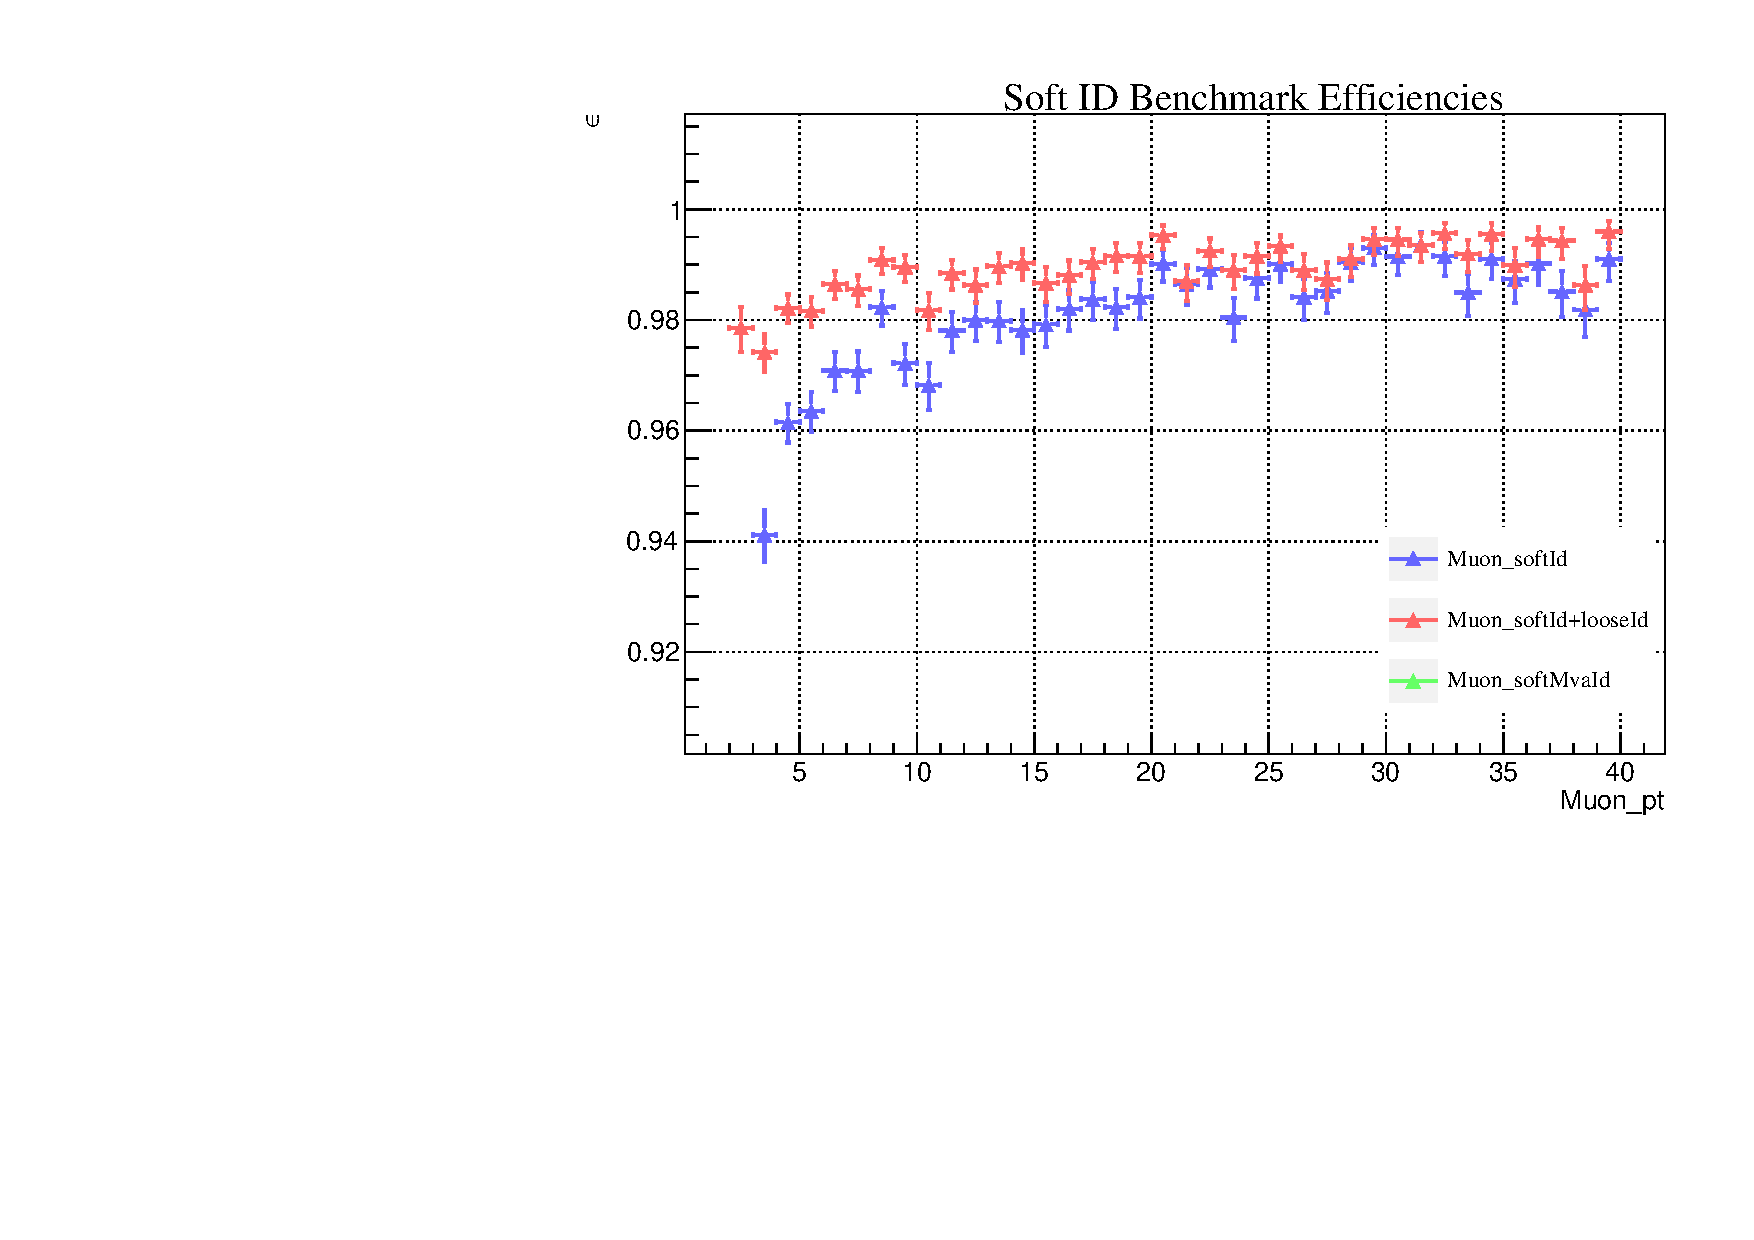
\includegraphics[scale=.5]{benchmarkEfficiency_TTjetszoomed.pdf}

$\epsilon$ = \# true muons that pass ID/\# true muons
\end{frame}

\begin{frame}{Results: Multiclass Classifier}
\centering
\includegraphics[scale=0.6]{model5_ROCcurveszoom.pdf}
\end{frame}

\begin{frame}{Results: Multiclass Classifier}
\centering
\includegraphics[scale=0.6]{model7_ROCcurveszoom.pdf}
\end{frame}









\end{document}